\documentclass[xcolor={dvipsnames}]{beamer}
\usepackage{color, colortbl}
\usepackage{transparent}
\usepackage[ngerman,english]{babel}
\usepackage[T1]{fontenc}
\usepackage{lmodern}
%\usepackage{subfigure}
%\usepackage[compatibility=false]{caption}
%\usepackage{subcaption}
\usepackage{tikz}
\usepackage{textgreek}
\usepackage{tabularx}
\usepackage{booktabs}
\usepackage{siunitx}
\usepackage{units}

\mode<presentation>
{
  \usetheme{CambridgeUS}     
  \usecolortheme{lily} 
  \definecolor{beamer@violet}{rgb}{0.5,0.3,0.5} % changed this
  \setbeamercolor{structure}{fg=beamer@violet!70!cyan}
  \setbeamercolor{palette primary}{fg=black, bg=gray!30!white!50!cyan!20!}
  \setbeamercolor{palette secondary}{fg=black, bg=gray!30!white!30!cyan!40!}
  \setbeamercolor*{palette tertiary}{bg=gray!20!white!20!cyan!60!}
  
  \setbeamercolor{frametitle}{fg=cyan!60!white!40!,bg=cyan!80!black}
  \setbeamercolor{title}{fg=cyan!80!black}
  \setbeamercolor{normal text}{fg=black,bg=white}
  \setbeamercolor{alerted text}{fg=beamer@violet}
  \setbeamercolor{example text}{fg=beamer@violet!70!cyan}
  
  \usefonttheme{structureitalicserif} 
  \setbeamertemplate{navigation symbols}{}
  \setbeamertemplate{caption}[numbered]
} 

\title[ILC \& Muons from spoilers]{\textbf{\LARGE The International Linear Collider \\ \small Muons from the muon spoilers in the SiD detector - FIRST RESULTS}}
\author{\textbf{Anne Sch\"utz}}
\institute{\textbf{DESY}}
\date{\textbf{23rd September 2016}}

\titlegraphic{
\includegraphics[height=1.0cm]{SiD.jpeg}\hspace*{6cm}~%
   
\includegraphics[height=1.0cm]{DESY_Logo.png}
}

\begin{document}
{
\usebackgroundtemplate{
 \tikz\node[opacity=0.1]{\hspace*{-.05in}\vspace*{-4in}{\transparent{0.1}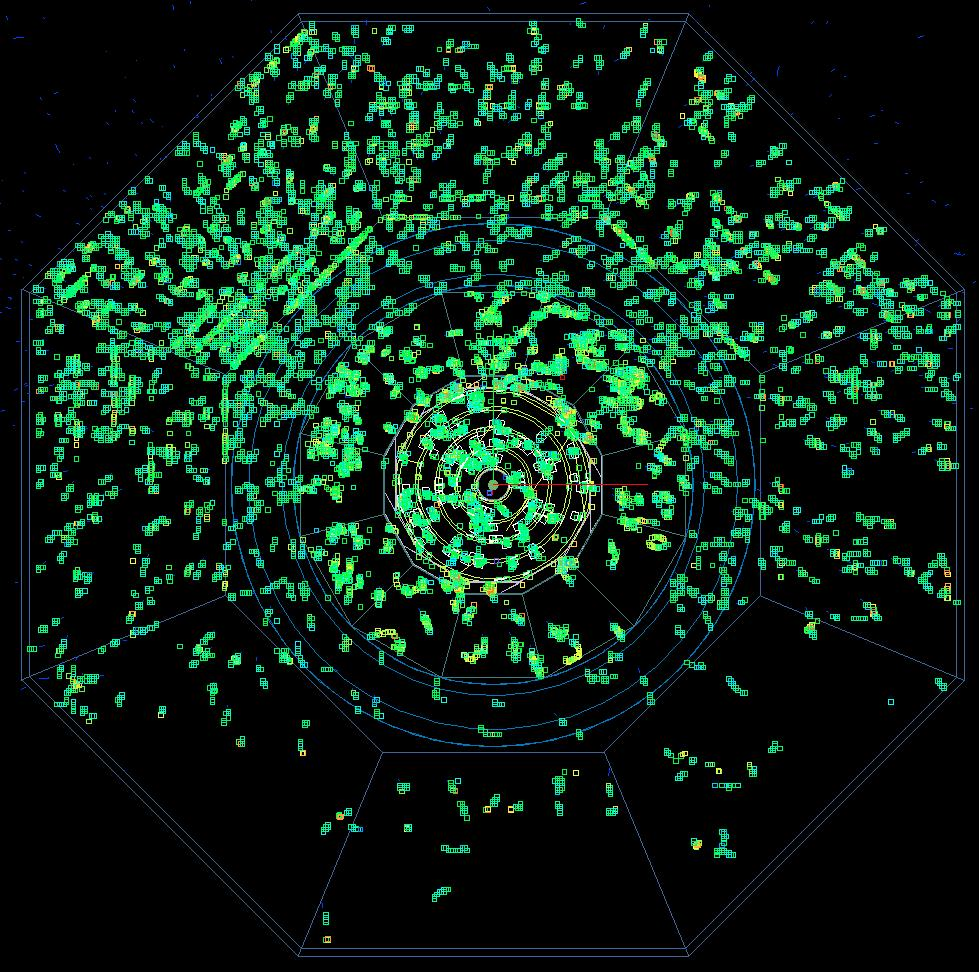
\includegraphics[width=\paperwidth]{muons_eventdisplay.jpeg}}};
 % \tikz\node[opacity=0.2]{\centering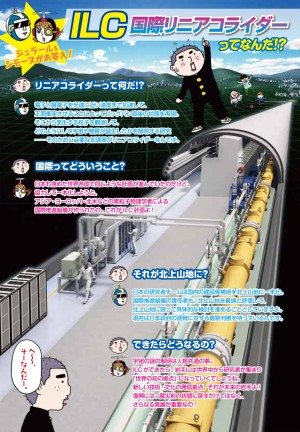
\includegraphics[height=\paperheight]{Iwatecomics.jpg}};
 }
\begin{frame}
  \titlepage
\end{frame}
}
\begin{frame}
  \tableofcontents
\end{frame}

\section{Muons from the muon spoilers}
\begin{frame}{BDS tunnel layout}
\begin{center}
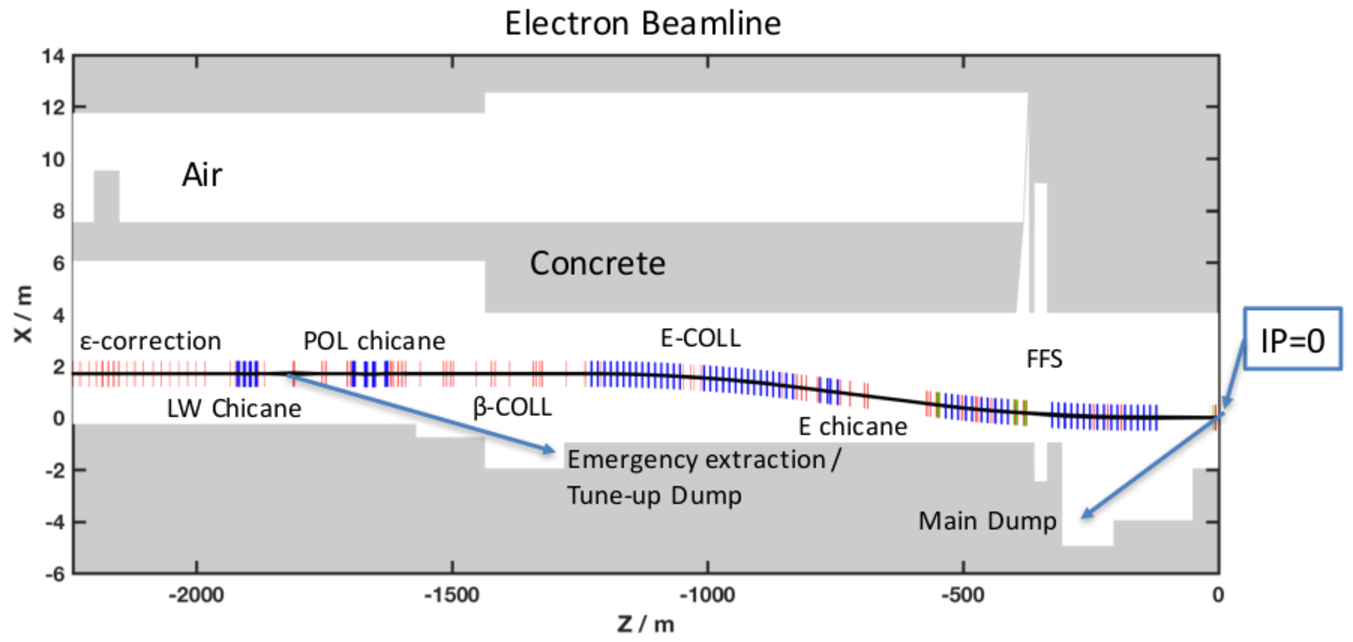
\includegraphics[height=0.65\textheight]{BDS_electron_tunnel.pdf}
\end{center}
\end{frame}

\subsection{Muon spoiler scenarios}
\begin{frame}{Muon spoiler scenarios}
There are two spoiler scenarios under discussion:
\begin{itemize}
 \item 3 donut spoilers
 \item 3 donut spoilers + wall
\end{itemize}
\begin{center}
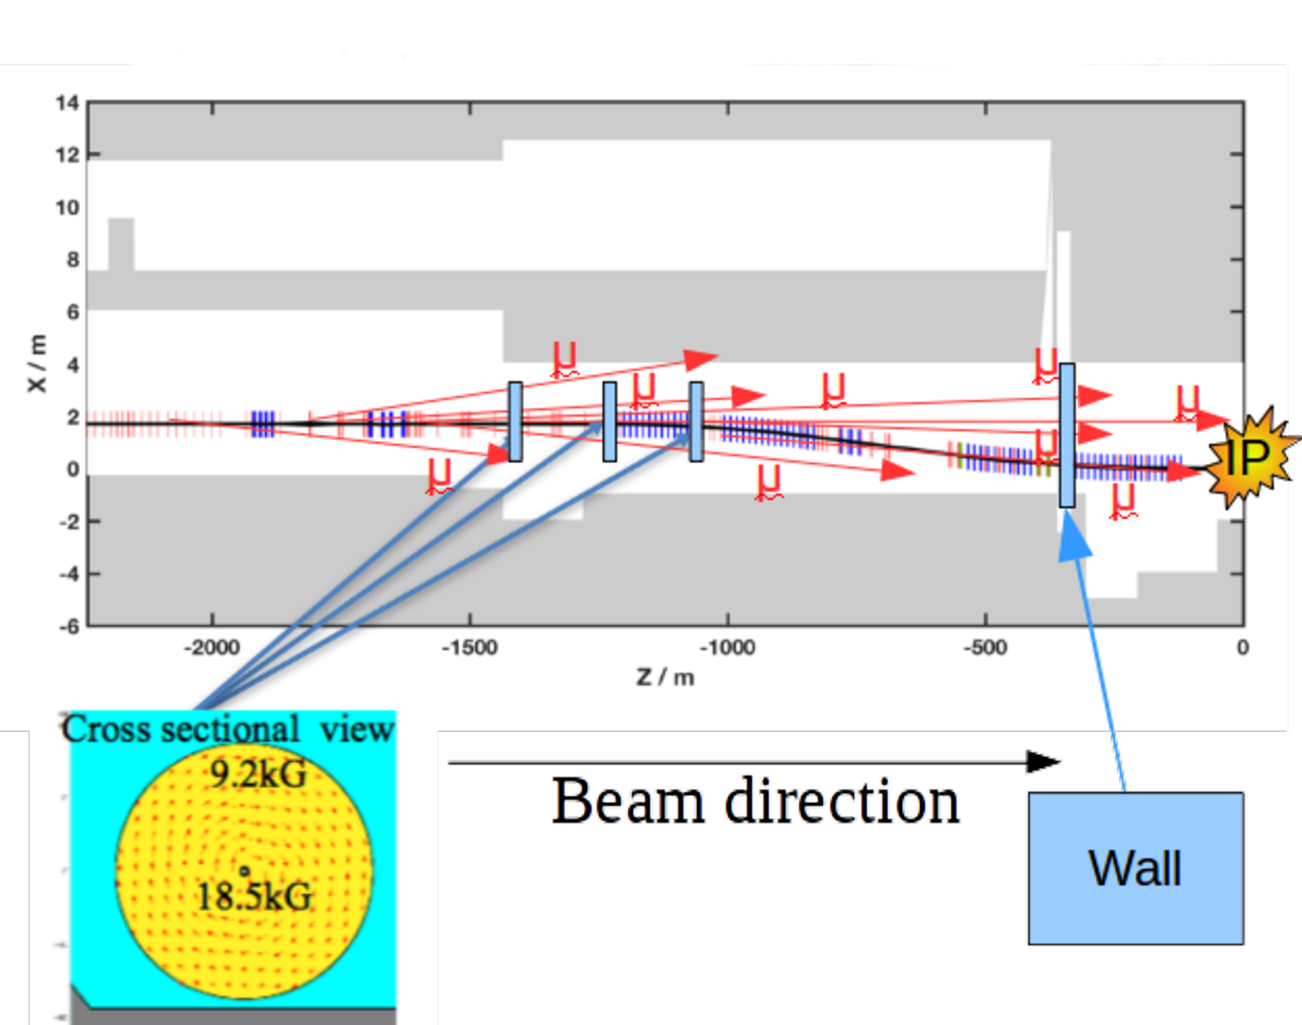
\includegraphics[height=0.7\textheight]{Muon_spoiler_scenarios.pdf}
\end{center}
\end{frame}

\begin{frame}{3 donut spoilers}
\textbf{The donut spoilers} are designed as follows:
\begin{itemize}
 \item \unit[70]{cm} radius
 \item \unit[5]{m} long
 \item Magnetized  with a field of $\sim$\unit[10-19]{kG}
\end{itemize}
\begin{center}
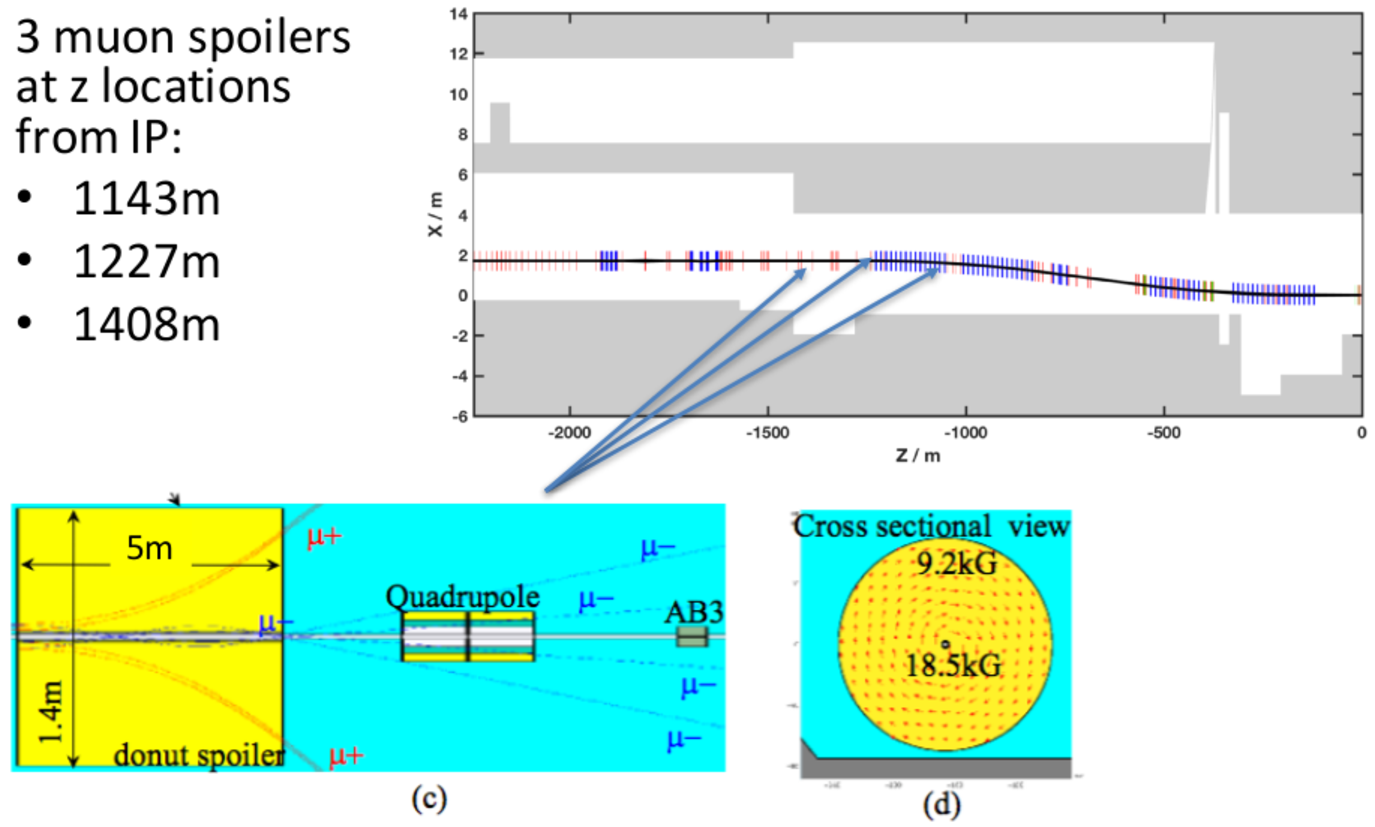
\includegraphics[height=0.67\textheight]{Muon_spoilers.pdf}
\end{center}
\end{frame}

\begin{frame}{3 donut spoilers + wall}
\textbf{The steel wall} would completely fill up the tunnel:
\begin{itemize}
 \item \unit[5]{m} x \unit[3]{m}, \unit[5]{m} long
 \item Magnetized with a field of $\sim$\unit[16]{kG}
 \item Located $\sim$\unit[400]{m} away from the IP
 \item Would cost $\sim$ \$3 million
\end{itemize}
\begin{center}
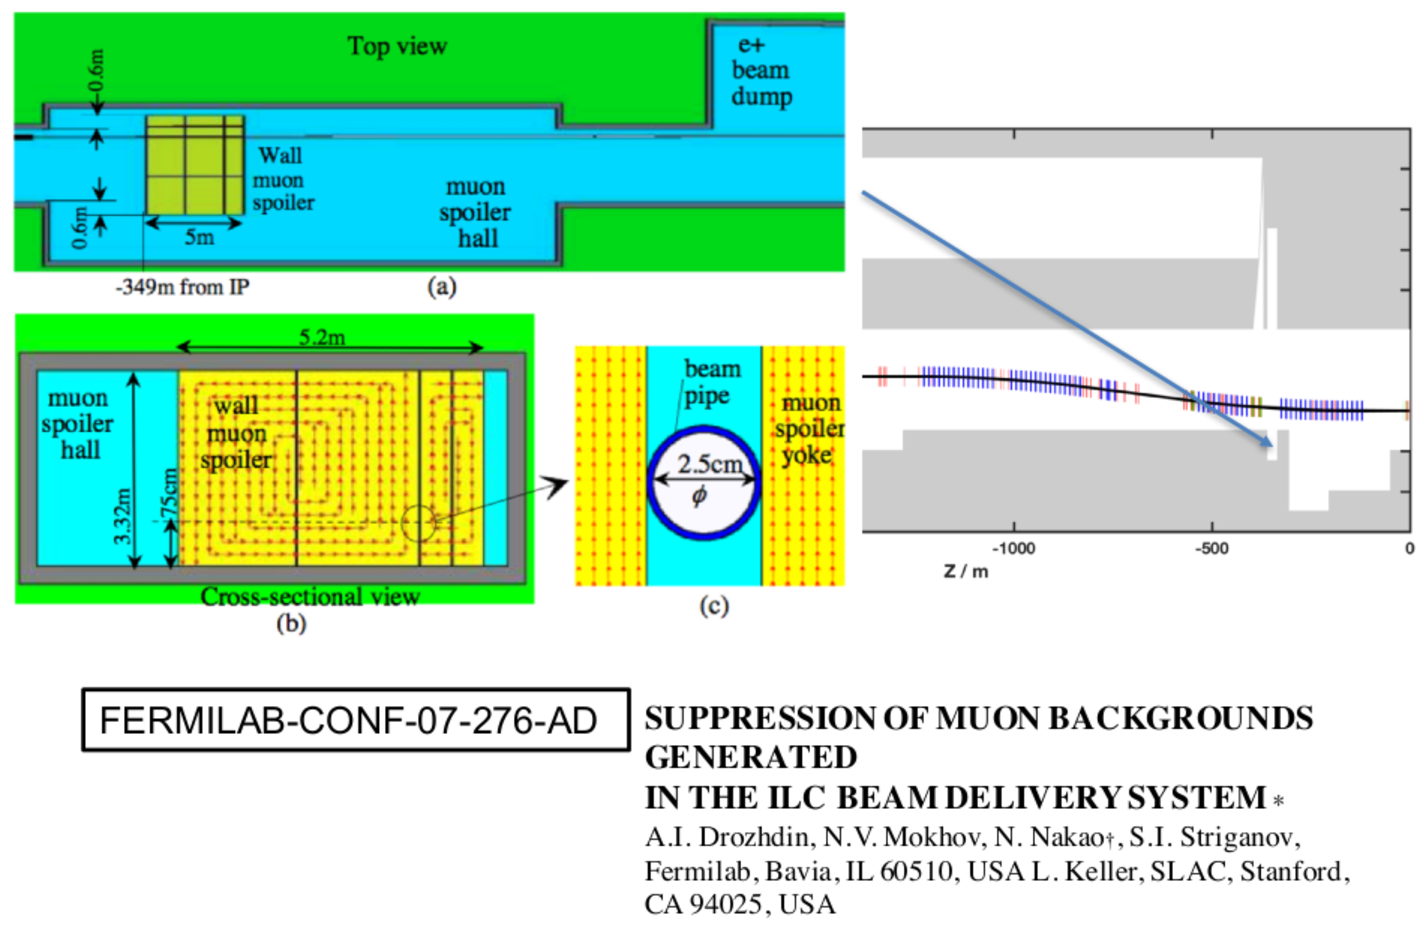
\includegraphics[height=0.7\textheight]{Muon_wall.pdf}
\end{center}
\end{frame}

\section{MUCARLO simulation}
\begin{frame}{MUCARLO simulation overview}
\begin{itemize}
\item BDS backgrounds with muon collimation system modelled with MUCARLO [Lewis Keller, SLAC] and Geant4 [Glen White, SLAC]
\item Using TDR baseline machine parameters for the ILC500
\item Muon production processes:
\begin{itemize}
\item Predominantly: Bethe-Heitler process: \textgamma + A $\rightarrow$ A' + \textmu$^+$\textmu$^-$
\item Few \% level: direct annihilation of positrons with atomic electrons: e$^+$e$^-$ $\rightarrow$ \textmu$^+$\textmu$^-$
\end{itemize}
\item Halo particle tracking:
\begin{itemize}
\item Turtle with MUCARLO
\item Lucretia with a built-in Geant4 model interface
\end{itemize}
\end{itemize}

\end{frame}

\subsection{Muon tracking}
\begin{frame}{Muon tracks in the BDS tunnel}
Muon tracks of positively (\textcolor{green}{\textmu\textsuperscript{+}}) and negatively( \textcolor{red}{\textmu\textsuperscript{-}}) charged muons, originating at two different primary betatron collimators: SP2 and SP4.
\begin{center}
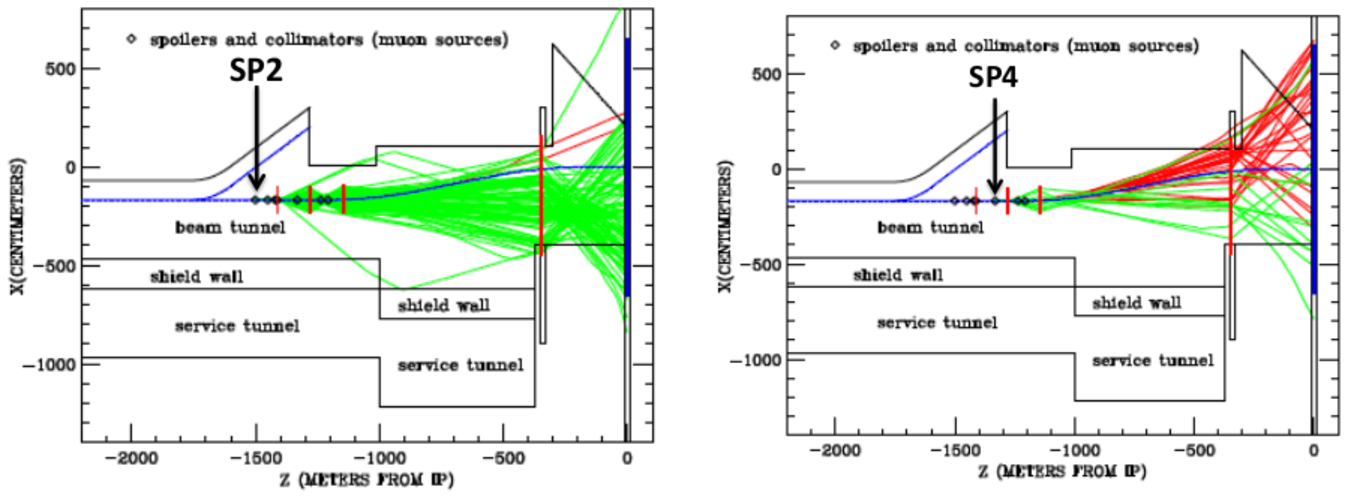
\includegraphics[width=0.95\textwidth]{Muon_tracks.pdf}
\end{center}
\end{frame}

\subsection{Muon 4-vectors}
\begin{frame}{Muon 4-vectors}
\begin{center}
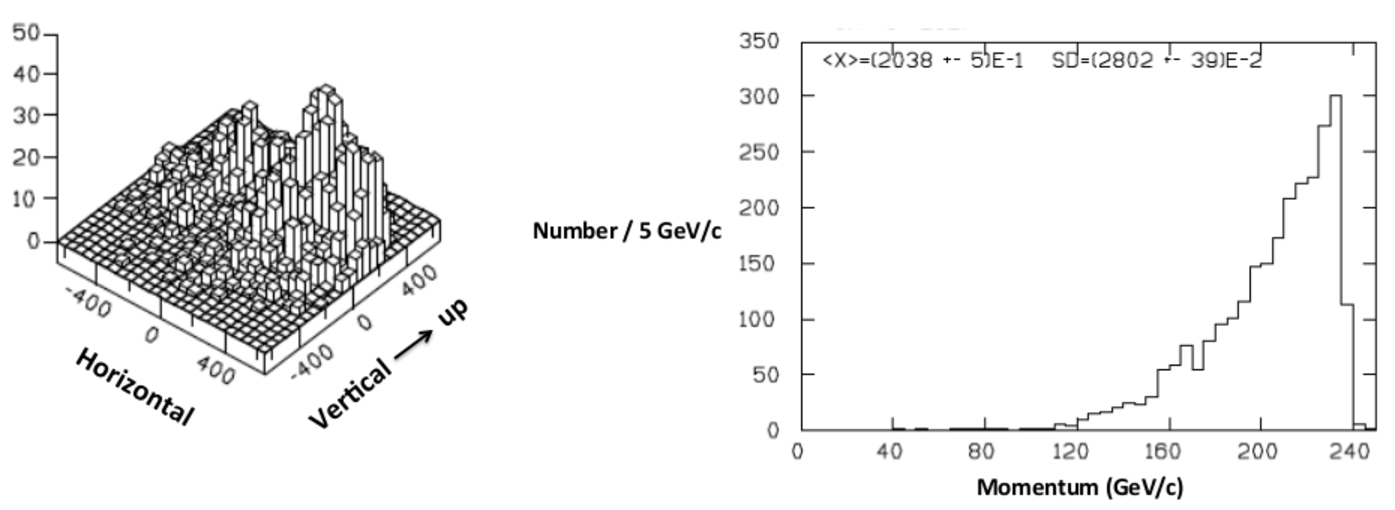
\includegraphics[height=0.5\textheight]{Muon_4-vectors.pdf}
\end{center}
Spatial and momentum distribution of muons in a detector (of 6.5m radius).
4-vectors provided to SiD and ILD.
\end{frame}
\begin{frame}{Muons in the detector}
\begin{center}
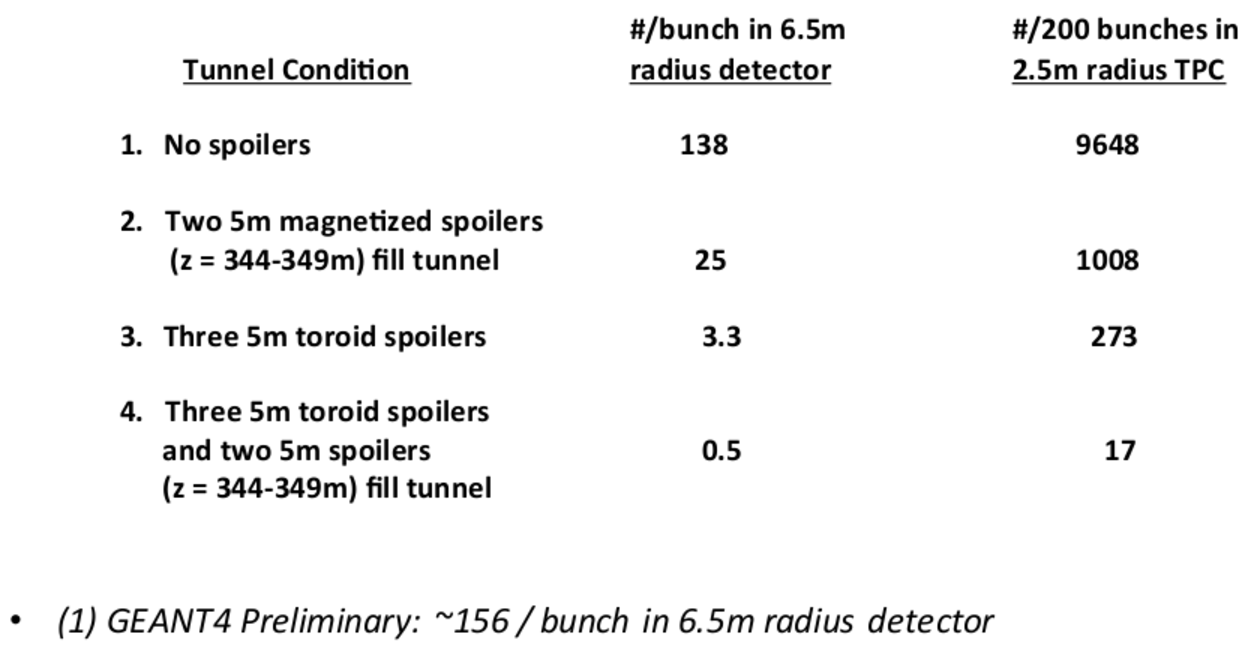
\includegraphics[height=0.6\textheight]{Muon_numbers.pdf}
\end{center}
First column: muon numbers per bunch in a detector with 6.5m radius.
The number can be reduced to below 1!
\end{frame}

\begin{frame}{Muons in the detector}
\begin{center}
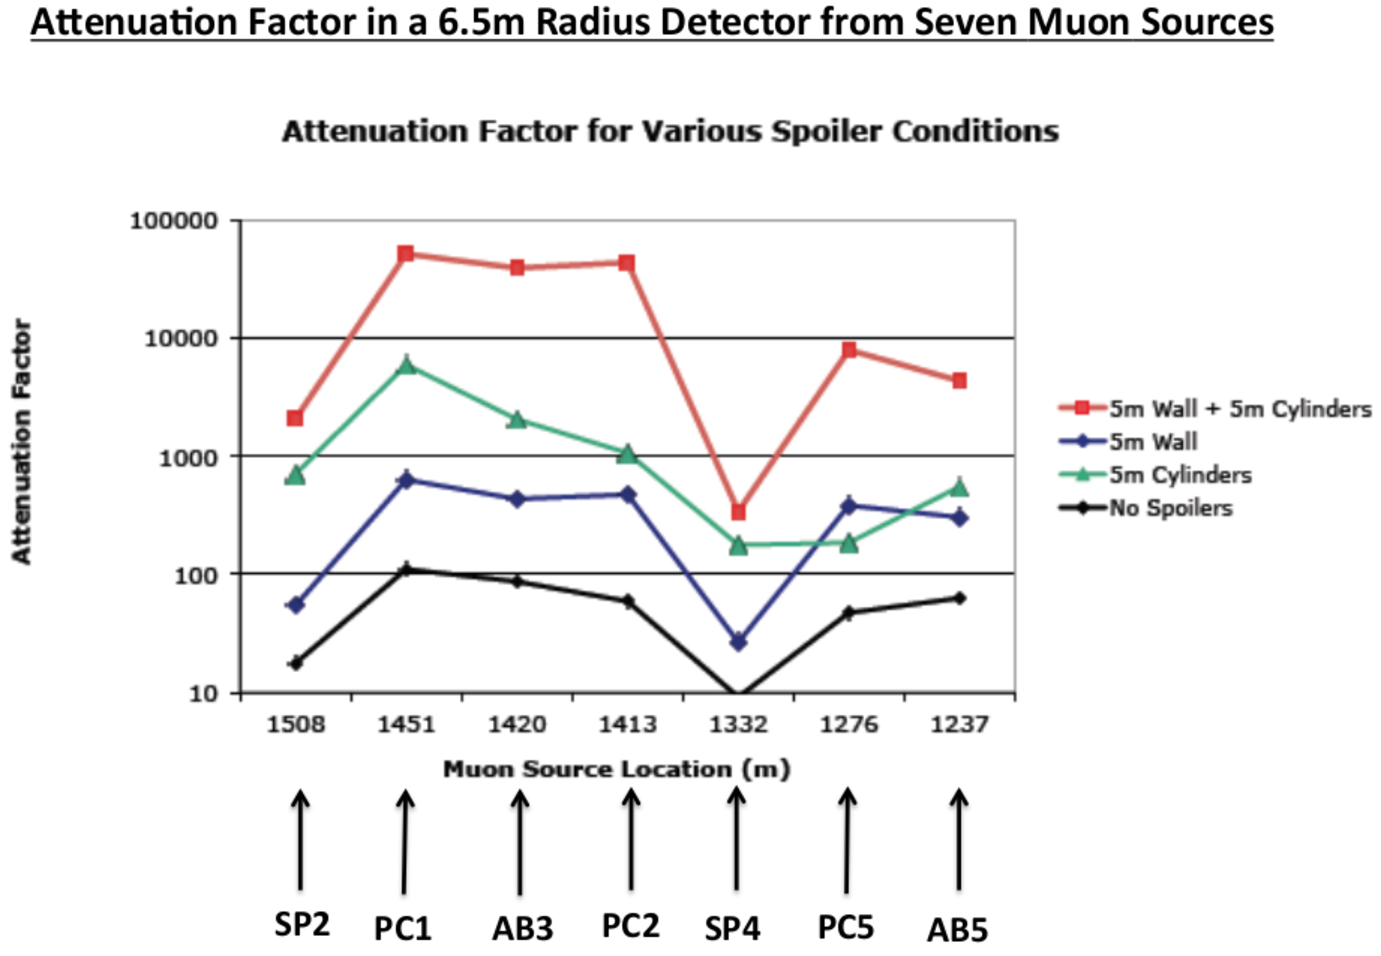
\includegraphics[height=0.7\textheight]{Attenuation_Factors.pdf}
\end{center}
The ratio of muons produced over muons which reach the detector, for different spoiler conditions and different source locations.
\end{frame}

\section{Motivation}
\begin{frame}{}
Question to SiD and ILD: Do we need the muon wall at all?!
MID people would be happy to get rid of it because of safety issues.
\begin{center}
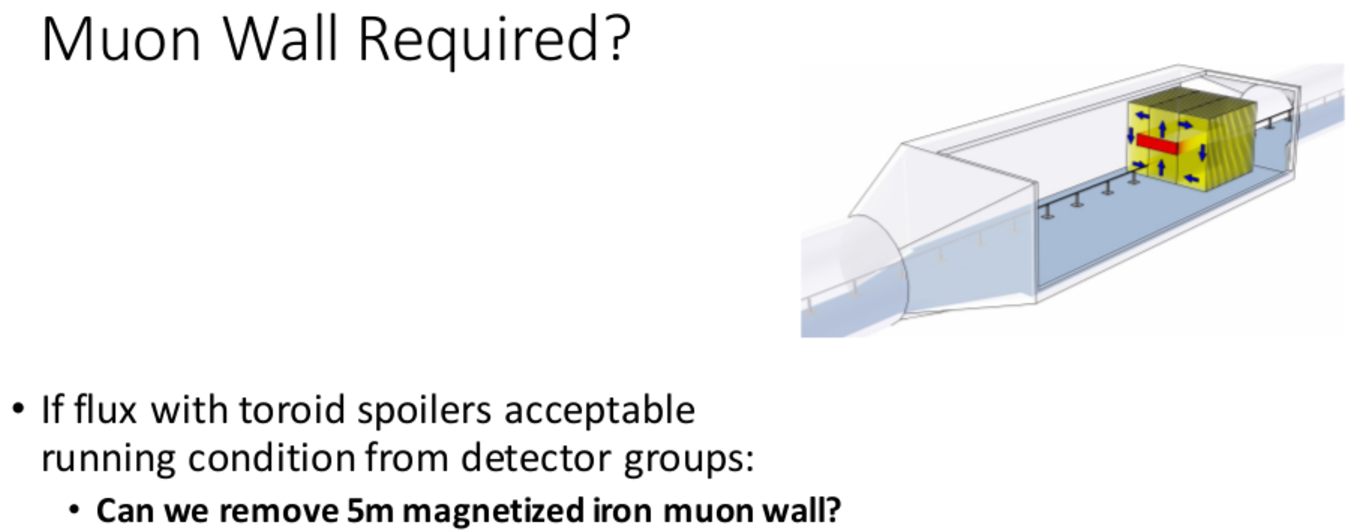
\includegraphics[height=0.5\textheight]{Muon_wall_required.pdf}
\end{center}
\end{frame}

\section{First results}
\begin{frame}{Summer student project}
The first analysis of the muon hits and the detector occupancy in the SiD detector was done by Jonas Glombitza, Marcel's and my summer student this summer 2016.\\
\vspace*{0.5cm}
Preparations:
\begin{itemize}
\item 4-vector files from Lewis Keller:
\begin{itemize}
 \item Spoilers + wall: from electron line: $\sim$1500 muons
 \item Spoilers + wall: from positron line: $\sim$2100 muons
 \item Spoilers: from electron line: $\sim$1080 muons
 \item Spoilers: from positron line: $\sim$2280 muons
\end{itemize}
\item Conversion of the text files with the 4-vector values to  STDHEP files of 1 train worth of muons.
\item The STDHEP files were used as input to a full SiD detector simulation with SLIC.
\item Nice event displays from the simulations with WIRED4 in JAS3.
\end{itemize}

\end{frame}

\subsection{Event displays of muons in the SiD detector}
\begin{frame}{WIRED4 event display}
1 train worth of muons ($\sim$ 650 muons):
\begin{center}
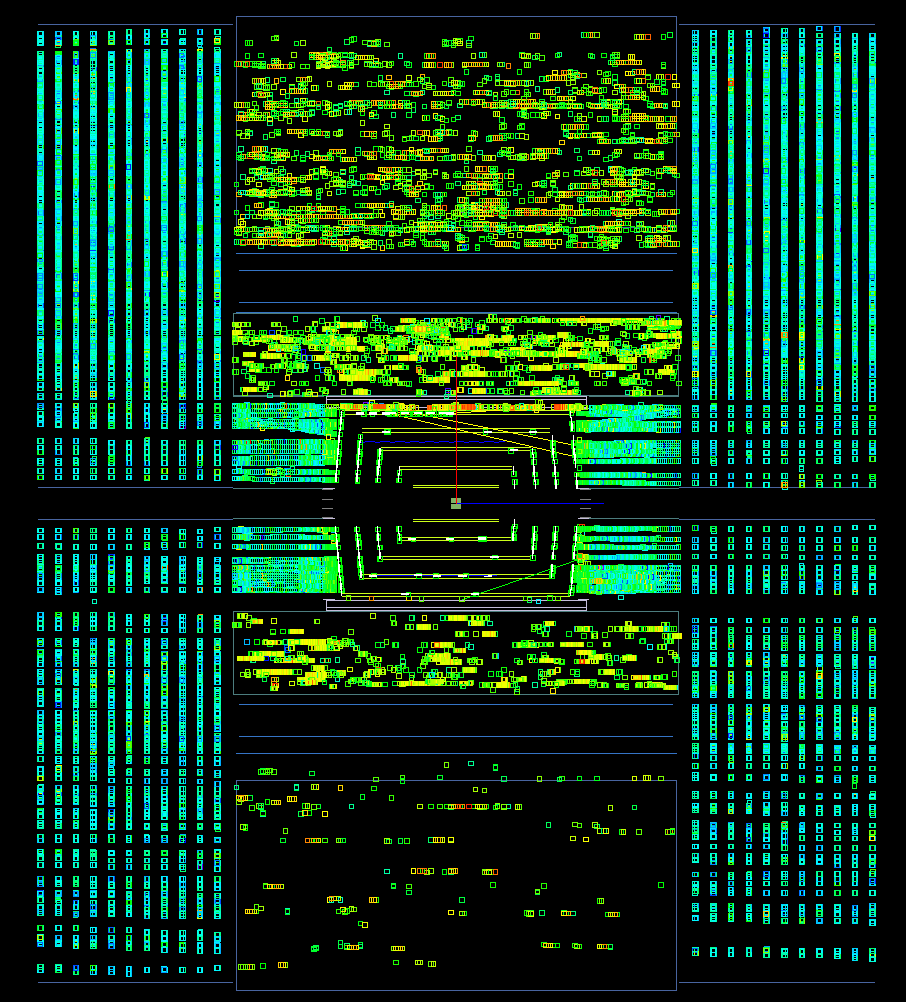
\includegraphics[height=0.6\textheight]{sidloi3_muons_wired4_eventdisplay_1bunch.png}
\hspace*{0.2cm}
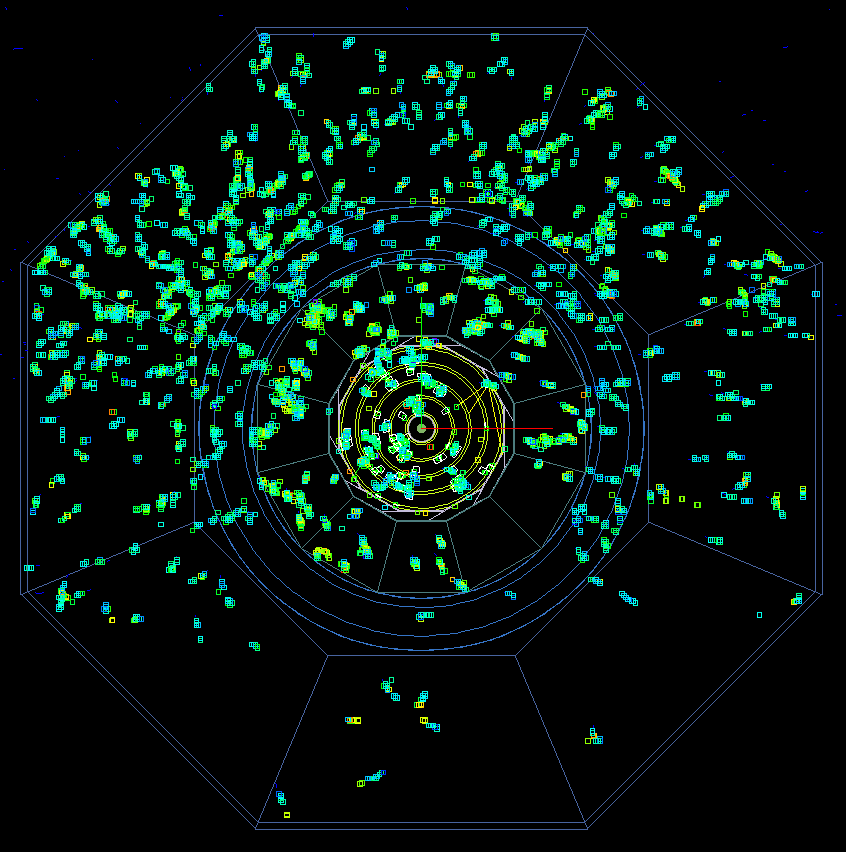
\includegraphics[height=0.6\textheight]{sidloi3_muons_wired4_eventdisplay_xy_view_1bunch.png}
\end{center}
The asymmetry in the xy plane is predicted by the MUCARLO simulation output (see a few slides before), and clearly visible also in the SLIC simulation.
\end{frame}

\subsection{Analysis}

\section{Conclusion and Outlook}
\begin{frame}
\textit{Conclusion:}
\begin{itemize}
\item Low energy muons are stopped by the muon wall.
\item High energy muons could be used for tracker alignment.
\end{itemize}
\textit{Outlook:}
\begin{itemize}
\item Need to wait for more files from Lewis. He is cross-checking his results with Glen White at the moment.
\item The timing information need to be updated.
\item Finalizing statement about absolute numbers of muons in both scenarios (spoilers, spoilers + wall), and about detector occupancies
\end{itemize}
\alert{Maybe a final conclusion about whether a muon wall is needed will have to wait till then...\\
$\rightarrow$\textit{Stay tuned!}}
\end{frame}

\section{References}
\begin{frame}{References}
\tiny
\begin{thebibliography}{9}
\setbeamertemplate{bibliography item}[text]
\bibitem{MUCARLO_talk}  \emph{ECFA 2016: Talk by Glen White about the MUCARLO simulation of the muons from the muon spoilers}. \url{https://agenda.linearcollider.org/event/7014/contributions/34689/attachments/30076/44961/ILC_muons.pptx}
\bibitem{Jonas_talk}  \emph{DESY summer student program: Talk by Jonas Glomitza (RWTH Aachen) about ``The Impacts of the Muon Spoiler Background on the ILC Detector Performance'', 08. September 2016}. \url{https://indico.desy.de/getFile.py/access?contribId=9&resId=0&materialId=slides&confId=15972}
\bibitem{Suppression}  \emph{FERMILAB-CONF-07-276-AD: ``Suppression of Muon Backgrounds generated in the ILC Beam Delivery System'', Drozhdin et.al, 2007}. \url{https://inspirehep.net/record/771808/files/fermilab-conf-07-276.pdf}
\bibitem{MUCARLO}  \emph{``Calculation of Muon Background in Electron Accelerators using the Monte Carlo Computer Program MUCARLO'', Rokni et.al}. \url{http://www.slac.stanford.edu/cgi-wrap/getdoc/slac-pub-7054.pdf}
\bibitem{MuonBackground_1TeV}  \emph{SLAC-PUB-6385: ``Muon Background in a 1.0-TeV Linear Collider'', L.P. Keller, 1993}. \url{http://www.slac.stanford.edu/pubs/slacpubs/6250/slac-pub-6385.pdf}
\bibitem{MuonBackground_0.5TeV}  \emph{SLAC-PUB-5533: ``Calculation of Muon Background in a 0.5 TeV Linear Collider'', L.P. Keller, 1991}. \url{http://www.slac.stanford.edu/cgi-wrap/getdoc/slac-pub-5533.pdf}
\end{thebibliography}
\end{frame}
%%--------------------------------------------------------------------------------

\end{document}
